\section{Stonk Bench Architecture}
  \subsection{Datasets and Preprocessing}
    The preprocessing procedure builds upon the TSGBench pipeline, 
    which standardizes segmentation, normalization, and train/test 
    splitting of the time series \cite{Ang23}. Several
    modifications were introduced to better accommodate financial
    time series and stochastic models.

    \subsubsection{Data type.} Stock price data at 
      daily frequency at closing price are 
      used. Let \(X \in \mathbb{R}^{L}\) denote a 
      time series with \(N=1\) channel(s) and length 
      \(L\).

    \subsubsection{Transformations.}\label{sec:transformations}
      Raw prices are converted to log-returns per channel via

      \[ r_t = \log S_t - \log S_{t-1} = \log(S_t / S_{t-1}) \,, 
      \quad r_t \in \mathbb{R^T}, \]
      
      yielding a transformed series of length \(L-1\). Log returns 
      are preferred in finance due to their variance-stabilizing 
      properties, preserving heavy tails and volatility clustering,
      and removal of the first order integration (random walk) 
      commonly exhibited in price series \cite{Takahashi24}.

    \subsubsection{Sequence lengths specification}\label{sec:sequence_length}
      To address research question \ref{rq:1}, we 
        experiment with varying training sequence lengths \(L\).
        For deep learning models, overlapping sliding windows 
        \(\mathcal{W} \in \mathbb{R}^{R \times L \times N}\) with 
        stride 1 are extracted.
        Specifically, we consider the following lengths \( L \):
        60, 120, 240, 300 minutes, and the maximum significant 
        partial autocorrelation lag.
      
      Unlike TSGBench, which employs an 
        autocorrelation-based hard-coded window of 125 (often 
        yielding a size of 1 for financial returns due to fast 
        autocorrelation decay \cite{Takahashi24,Cont01}), the window
        length \(L\) is alternatively
        determined via the partial autocorrelation function (PACF).
        The PACF aims to remove indirect correlations from in-between
        lags due to auto-regressive structures by finding the 
        best linear-predictor of the intermediate lagged values
        \cite{Durbin60}. Particularly for a lag \(h\), the PACF
        \(\phi_{hh}\) is defined between \( X_t \) and \( X_{t+h}\) as
        \begin{equation*}
        \phi_{hh} = \text{corr}\bigl(X_t - \hat{X}_t, X_{t+h} - \hat{X}_{t+h}\bigr),
        \end{equation*}
        where \(\hat{X}_t, \hat{X}_{t+h}\) is the best linear 
        predictor of \(X_t, X_{t+h}\),respectively, given the
        intermediate lags \(X_{t+1}, \ldots, X_{t+h-1}\).
        Specifically, PACF is computed up to 
        \(\lfloor 10\log_{10} n \rfloor\) lags (this value is determined
        from TSGBench \cite{Ang23}), and the lag 
        corresponding to the maximum significant PACF peak across 
        channels is selected, resulting in \(L=52\). This approach 
        captures relevant temporal dependencies within the data.

    \subsubsection{Model-specific preprocessing.}\label{sec:model-specific}
    The preprocessing follows the general TSGBench framework,
    with the following adaptations:

    \begin{itemize}
        \item Log returns are used directly instead of TSGBench's 
        min-max normalization for the reasons outlined in 
        §\ref{sec:transformations}. 
        \item For parametric models, the transformed series is 
        divided into contiguous training, validation, and test 
        segments with ratios \((1-\alpha-\beta):\alpha:\beta\), 
        where \(\alpha=0.1\) and \(\beta=0.1\). This ensures that 
        parametric models fit parameters directly to contiguous 
        historical data.
  
        \item The dataset is split into train, validation, and test 
        sets while preserving temporal order to prevent future 
        information from leaking into the past. Only the training 
        set is shuffled during model training to improve 
        convergence. In contrast, TSG-Bench shuffles time series 
        samples before splitting, which introduces data leakage. 
        Our approach ensures strictly forward-looking evaluation 
        for realistic forecasting.

        proper evaluation, consistent with TSGBench.
    \end{itemize}

    \subsubsection{Data loaders.} For deep learning models, 
    mini-batches are generated from the windowed data 
    \(\mathcal{W}\) using independent fixed seeds for training, 
    validation, and test sets, enabling reproducible epoch-wise 
    evaluation. Training batches are shuffled, while validation 
    and test sets maintain sequential ordering. To ensure fair 
    comparison, parametric models generate sequences of identical 
    length \(L\) and matching sample count to the windowed data 
    used by deep learning models.

        
      \end{enumerate}
  \subsection{Utility Evaluation Measures}\label{subsec:utility-measure}
    Utility measures are critical for evaluating synthetic data 
    beyond statistical metrics, as they assess the practical value 
    of generated data in real-world financial applications 
    \cite{Boursin22}. Our benchmark incorporates (deep) hedging as a 
    utility measure for several key reasons:

    \begin{enumerate}[label=\textbf{[U\arabic*]}]
      \item \label{utility:application}\textbf{Real-world 
      Application Testing:}
      (Deep) hedging provides a concrete way to evaluate how 
      synthetic data performs in actual financial tasks, 
      particularly in derivatives pricing and risk management.

      \item \label{utility:industry}\textbf{Industry-relevant 
      Metrics:}
      By comparing hedging strategies trained on synthetic versus 
      real data, we can assess the practical utility of synthetic 
      data through metrics that matter to financial practitioners, 
      such as replication errors and hedging performance.

      \item \label{utility:validation}\textbf{Model Robustness 
      Validation:}
      (Deep) hedging helps verify if synthetic data maintains the 
      complex relationships and market dynamics necessary for 
      developing reliable trading strategies.
    \end{enumerate}

    \subsubsection{(Deep) hedger Problem Defintion}
      We consider a continuous-time financial market defined on a 
      probability space $(\Omega, \mathcal{F}, \mathbb{P})$, over 
      a finite time horizon $0 < T < \infty$, equipped with a 
      filtration $\mathcal{F} = (\mathcal{F}_t)_{0 \leq t \leq T}$ 
      that represents the evolution of information through time.  
      The market consists of asset $S_t$. For simplicity, we assume a zero 
      interest rate environment.
      The asset \(S_t\) follow a stochastic differential
      equation. We focus on a single underlying asset \(S_t\), and we are
      concerned with hedging a European call option with strike price \(K\)
      and maturity \(T\) so the payoff is \(g(S_T) = \max(S_T - K, 0)\).

      We study the hedging problem associated with a contingent 
      claim delivering a payoff $g(S_T)$ at maturity $T$, where 
      $S_T$ represents the terminal value of the underlying asset 
      vector.  
      The hedging strategy is implemented at a discrete set of 
      times $0 = t_0 < t_1 < \dots < t_{N-1} < t_N = T$.  
      A \textit{self-financing portfolio} is described by a 
      $d$-dimensional $\mathcal{F}_t$-adapted process $\Delta_t$, 
      and its terminal wealth, denoted $X_T^{\Delta, p}$, is 
      given by
      \begin{equation}
          X_T^{\Delta, p} = p + \sum_{i=1}^{d} \sum_{j=0}^{N-1} 
          \Delta_{t_j}^i \left( F_{t_{j+1}}^i - F_{t_j}^i \right),
      \end{equation}
      where $p \in \mathbb{R}$ represents the initial premium.

      The objective is to determine the optimal premium and 
      trading strategy $(p^{\text{opt}}, \Delta^{\text{opt}})$ 
      that minimize the expected squared hedging error:
      \begin{equation}
          (p^{\text{opt}}, \Delta^{\text{opt}}) 
          = \operatorname*{Argmin}_{p, \Delta} 
          \mathbb{E} \left[ \big( X_T^{\Delta} - g(S_T) 
          \big)^2 \right].
      \end{equation}

      To address this optimization problem, we employ the global 
      approach proposed by Fécamp \textit{et al.} (2020), chosen 
      for its computational efficiency and scalability.  
      In this framework, the control policy $\Delta$ is 
      approximated by a feed-forward neural network—referred to as 
      a \textit{deep hedger}—which jointly learns the optimal 
      trading strategy and corresponding premium through 
      end-to-end training \cite{Fecamp20}.

      \begin{figure}[h]
        \centering
        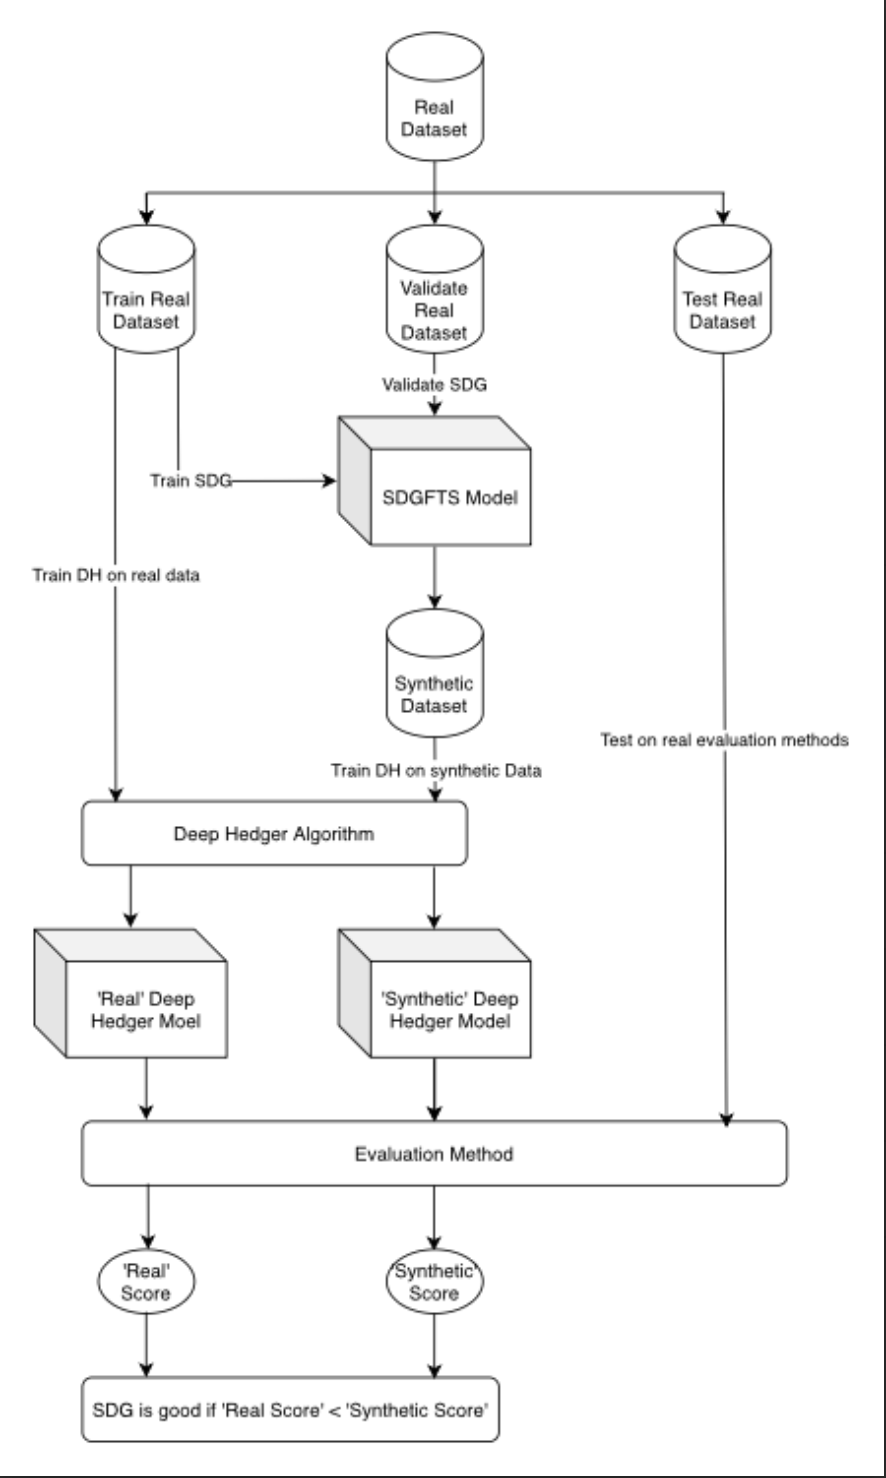
\includegraphics[width=0.3\textwidth,keepaspectratio]{../../results/deep_hedger_architecture.png}
        \caption{Architecture overview of the (deep) hedger evaluation framework, 
        illustrating the flow from data preparation through model training to 
        performance evaluation.}
        \Description{Diagram showing the complete pipeline of the deep hedger 
        architecture including data splits, model training, and evaluation steps.}
        \label{fig:deep_hedger_architecture}
      \end{figure}
    
  \begin{figure*}[h]
      \centering
      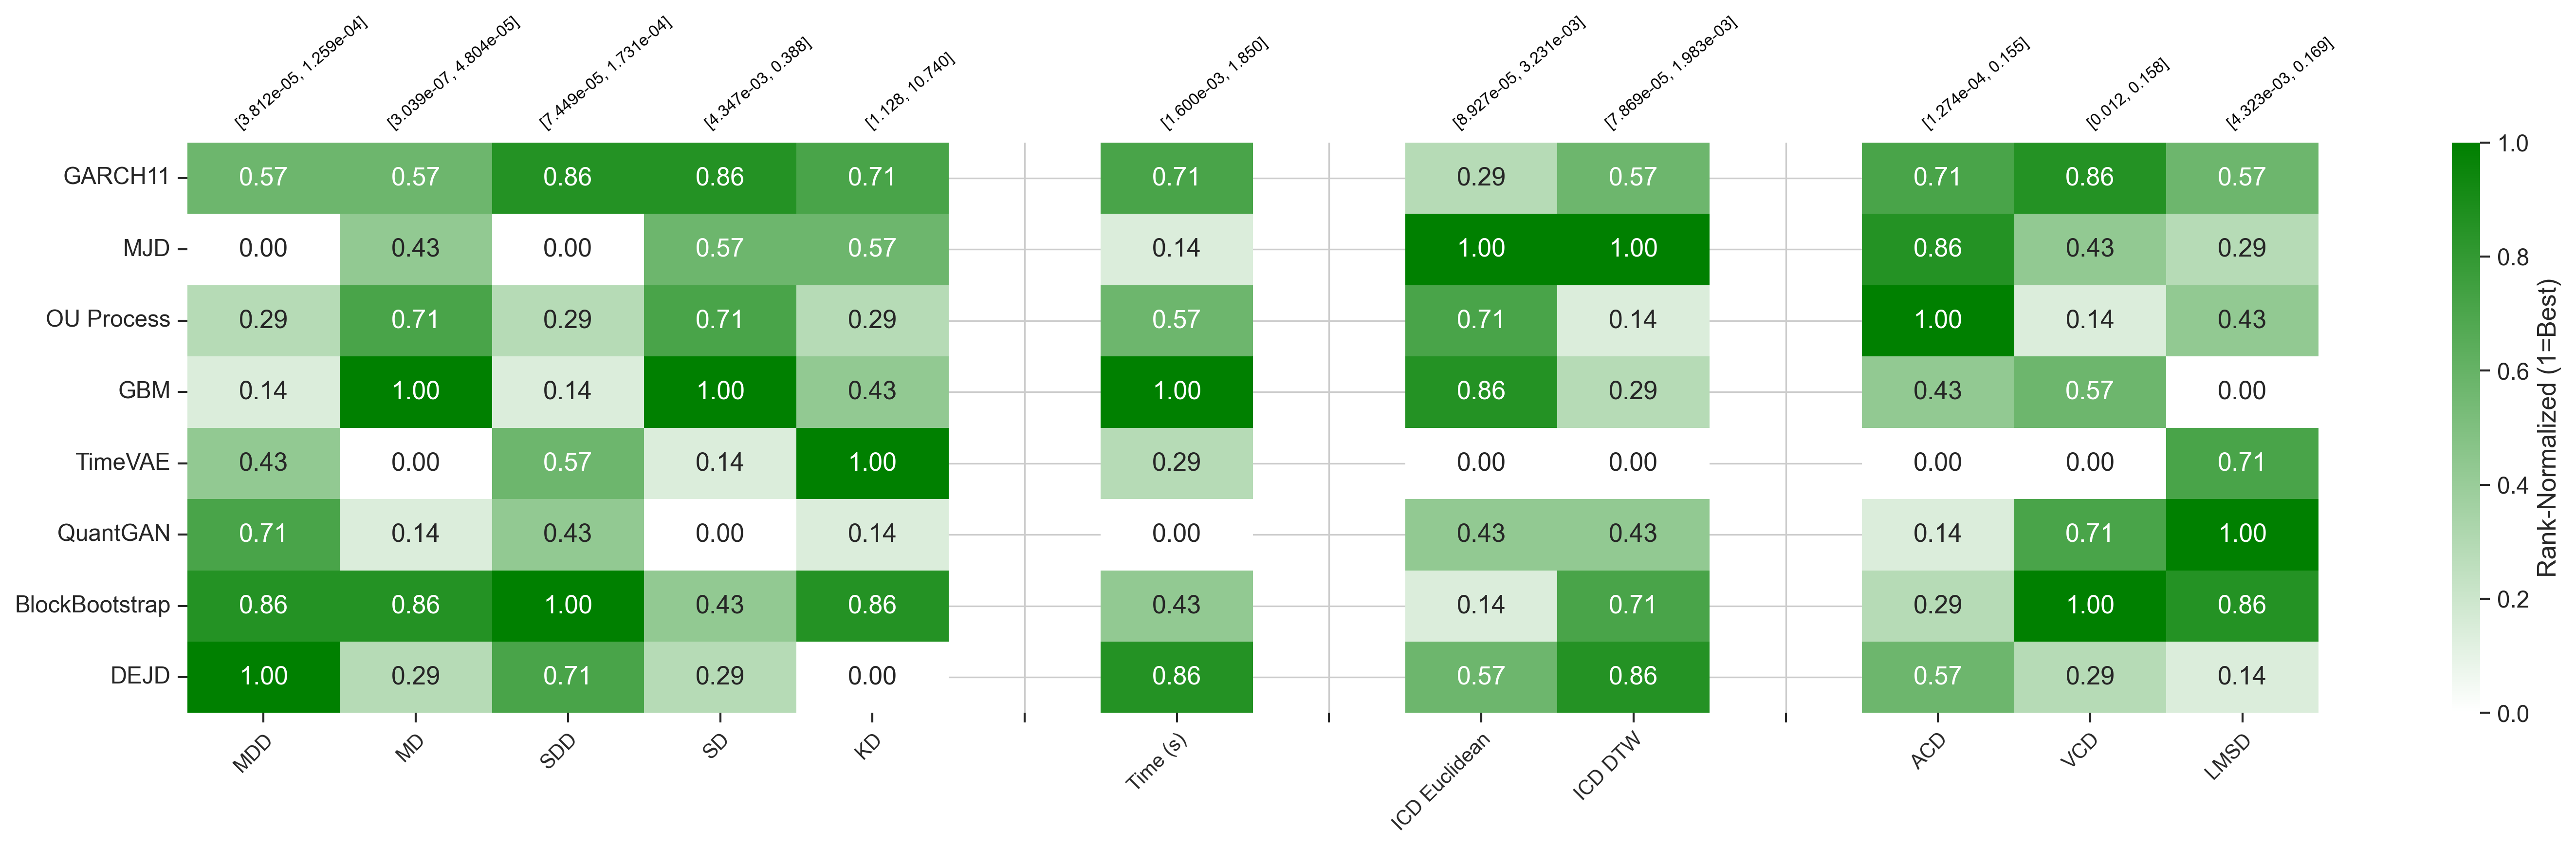
\includegraphics[width=\textwidth,height=8cm, keepaspectratio]
      {../../results/main_experiment/figure_1_per_metric_heatmaps/figure_1_all_taxonomies_ranknorm_heatmap.png}
      \caption{Normalized ranking heatmap across all evaluation 
      taxonomies.
      For diversity metrics, a score of (1) indicates
      highest metric value (most diverse), while for other metrics,
      a score of (1) indicates lowest metric value (best performance).
      Raw minimum and maximum values are provided for each metric on 
      top of each respective column.
      (Specification: sequence length based on
      maximum significant PACF lag)}
      \Description{The heatmap displays the normalized rankings of various
      models across different evaluation metrics.}
      \label{fig:heatmap_all_taxonomies}
  \end{figure*}
  
    \subsubsection{(Deep) hedger Architecture}
    %   \begin{table}[h]
    %     \centering
    %     \caption{Notations for (deep) hedger architecture.}
    %     \label{tab:deephedger-notation}
    %     \begin{tabular}{ll}
    %     \toprule
    %     \textbf{Symbol}     & \textbf{Description} \\
    %     \midrule
    %     \( D \)             & Time-series dataset             \\
    %     \( T \)             & Task                            \\
    %     \( S \)             & Score                           \\
    %     \( A \)             & (deep) hedger algorithm           \\
    %     \( \mathcal{A}_n \) & Set of n (deep) hedger algorithms \\
    %     \( M \)             & (deep) hedger model               \\
    %     \( \mathcal{M}_{TS} \)   & (SDGFTS) model                  \\
    %     \bottomrule
    %     \end{tabular}
    %   \end{table}

      Our (deep) hedger architecture centers around the 
      Train-Synthetic-Test-Real (TSTR) evaluation framework 
      \cite{Leznik21}, adapted for financial time series 
      generation. We begin with our real FTS dataset 
      \( D\)\textemdash partitioned to a training, validation, 
      and test set respectively as
      \( D_r = \{D_r^{train}, D_r^{validate}, D_r^{test}\} 
      \)\textemdash along with a specific hedging task \(T\) and a 
      performance score \(S\) to evaluate hedging effectiveness, to 
      which we will go indepth in the next subsubsection.
      We consider a (deep) hedger algorithm \(A\) (e.g. a 5-layer 
      perceptron) that takes as input the dataset \(D_r\) and 
      task \(T\),

      In the context of SDGFTS evaluation, we consider a SDGFTS 
      model \( \mathcal{M}_{TS} \) trained on \( D_r^{train} \) 
      and validated with \( D_r^{validate} \) to generate synthetic 
      FTS data \( D_g \).

      Now we can train a (deep) hedger algorithm \( A \) on the 
      datasets \( D_r^{train} \) and \( D_g^{train} \) 
      respectively, resulting in two (deep) hedger models
      \( M_r \) and \( M_g \).

      Finally, we evaluate both models on the real test set 
      \( D_r^{test} \) to obtain the corresponding performance 
      scores \( s_r \) and \( s_g \).

      The goal of the (deep) hedger portfolio evaluation is to 
      evaluate the effectiveness of the model 
      \( \mathcal{M}_{TS} \) with downstream tasks (hedging) 
      by comparing the scores \( s_r \) and \( s_g \). The model 
      \( \mathcal{M}_{TS} \) is considered effective if the 
      the results yielded similar scores, i.e. 
      \( s_r \approx s_g \) \textemdash preferably having higher 
      performance with results of \( s_g > s_r \) \textemdash 
      indicating that the synthetic data generated by 
      \( \mathcal{M}_{TS} \) is useful for training a (deep) hedger.

      \subsubsection{Augmented Testing}
      \label{sec:augmented-testing}
      To better evaluate the performance of (deep) hedgers trained 
      on synthetic data, we train our (deep) hedger \( A \) on a 
      new dataset \( D_{aug} \) that combines both real training 
      data \( D_r^{train} \) and synthetic data \( D_g\). In 
      other words, we train model \( M_g \) on \( D_{aug} \) 
      where \( D_{aug} := D_r^{train} \cup D_g\).
      Then we proceed to evaluate scores between models
      \( M_g \) and \( M_r \) on the real test set, where 
      \( M_r \) is still trained on only real data 
      \( D_r^{train} \).
      This extension, inspired by Stenger et al. \cite{Stenger24}, 
      allows us to assess whether synthetic data provides additional 
      value when combined with real training data.


      \subsubsection{Algorithm Comparison}
      \label{sec:algorithm-comparison}
      Another extension is to compare multiple (deep) hedger 
      algorithms to determine the degree to which each algorithm 
      performs equally on generated data relative to other algorithms, 
      compared to their performance on real data.

      Given a set of \( n \) (deep) hedger algorithms 
      \( \mathcal{A}_n = \{ A_1, \ldots, A_n \} \), we train 
      each algorithm \( A_i \in \mathcal{A}_n \) on both real 
      training data \( D_r^{train} \) and synthetic data 
      \( D_g^{train} \) respectively, resulting in two sets of 
      (deep) hedger models \(\{M_r^1, M_r^2, \ldots, M_r^n\} \) 
      and \( \{M_g^1, M_g^2, \ldots, M_g^n\} \) and two ordered 
      sets of performance scores 
      \( s_r := \{s_r^1, s_r^2, \ldots, s_r^n\} \) and 
      \( s_g := \{s_g^1, s_g^2, \ldots, s_g^n\} \) respectively.

      We compare the relative performance of each 
      algorithm on real data versus synthetic data by computing 
      the Spearman's rank correlation coefficient \( r_S \) 
      \cite{Lin21} between the two score sets \( s_r \) and 
      \( s_g \):
      \begin{equation}
        \begin{aligned}
          r_S &= 1 - \frac{6 \sum_{i=1}^{n} ( \mathrm{rank}(s_r^i) 
          - \mathrm{rank}(s_g^i) )^2}{n(n^2 - 1)},
        \end{aligned}
        \label{eq:Spearman}
      \end{equation}
      where \( \mathrm{rank}(s_r^i) \) and 
      \( \mathrm{rank}(s_g^i) \) denote the ranks of scores 
      \( s_r^i \) and \( s_g^i \) within their respective sets.

      A high positive correlation (i.e., \( r_S \) 
      close to 1) indicates that the synthetic data 
      generated by \( \mathcal{M}_{TS} \) preserves the relative 
      performance of different (deep) hedger algorithms, suggesting 
      that the synthetic data is suitable for algorithm evaluation 
      and comparison.

      The (deep) hedger algorithms \( \mathcal{A}_n \) considered in 
      this benchmark can be found in appendix 
      \ref{appendix:deep-hedger-algorithms}.

      \subsubsection{(Deep) hedger Portfolio Evaluation}
      We evaluate the suite of hedger algorithms trained on 
      synthetic and real data using the portfolio replication error 
      or replication loss metric \cite{Boursin22}.



